\chapter{\label{intro}Introduction}
%%%%%


\Glspl{GW} were first predicted in 1915 as a consequence of Einstein's general theory of relativity \citep{einstein2005GrundlageAllgemeinen}.
They are theorised as ripples in the fabric of space-time.
The first observational evidence that \glspl{GW} exist came from observations of the Hulse-Taylor binary \citep{weisberg1981GravitationalWaves,weisberg2004RelativisticBinary}. 
This observation of a pulsar in a binary system showed that the periastron was reached slightly early after each orbit, implying that the pulsars orbit was decreasing with time. 
If the separation of two orbiting objects is decreasing then the system must be losing energy.
The loss in energy matched the \gls{GR} prediction which assumed the energy was lost to \glspl{GW}.
This gave hope of \glspl{GW} existence and helped lead the way to designing instruments which could directly detect them.
The first direct detection of gravitational waves was made in 2015 when the two \gls{LIGO} detectors in the US \citep{abbott2016ObservationGravitational} identified a signal from a \gls{BBH} system.
This was not only the first observation of a \gls{GW} but gave information on a yet unobserved astrophysical system.
This has since been followed by many more detections of \gls{BBH} signals involving \gls{LIGO} and Virgo including \citep{abbott2017GW170814ThreeDetector,theligoscientificcollaboration2020GW190425Observation}.
In 2017 the \gls{LIGO} detectors observed the first \gls{BNS} system \citep{abbott2017GW170817Observation} which had a corresponding electromagnetic counterpart.
This allowed verification of the source from optical counterparts and started the era of multi-messenger astronomy.
These detections opened up the field of gravitational wave astronomy, where many more detections are expected to give more information on the universe and objects within it.

As well as searching for \gls{BBH} and \gls{BNS} signals, there are many efforts to detector other types of \gls{GW} signals. 
This thesis focuses on efforts to search for a particular type of \gls{GW} which are thought to originate from rapidly rotating neutron stars.
In chapters \ref{intro} and \ref{searchcw} I will review introductory material. 
This includes a general introduction to the generation of \glspl{GW} in Sec.~\ref{intro:gravwaves} and their sources in Sec.~\ref{intro:sources}.
I will then introduce instruments used to detect \gls{GW} in Sec.~\ref{intro:detector}.
In Chapter \ref{searchcw} I will introduce the general model for \glspl{CW} and current methods used to detect them.
Chapters \ref{soap}, \ref{machine} and \ref{detchar} will go into detail about techniques developed by the author to search for \gls{CW} signals. 
Finally I will summarise this work and discuss future developments in chapter \ref{summary}.


%%%%%%%%%%%
%%%%%%%%%
\section{\label{intro:gravwaves}Gravitational waves}
%%%%%%%%%%%
%%%%%%%%%

In general relativity, gravity is thought of as the curvature of space-time and matter moves according to this curvature. 
The matter in the universe also has an effect on the curvature of the space-time.
The larger the mass of matter the more the space-time is distorted.
Space-time can generally be described by Einstein's field equations
\begin{equation}
\label{intro:gravwaves:efe}
    G_{\mu \nu} = \frac{8 \pi G}{c^4}T_{\mu \nu}.
\end{equation}
where $G_{\mu \nu}$ is the Einstein tensor and $T_{\mu \nu}$ is the stress-energy tensor.
The stress energy tensor essentially describes the mass-energy in the universe, where its components contain information on the density of energy and momentum.
The Einstein tensor contains information on the curvature of the universe. 
This can be derived directly from the metric tensor $g_{\mu \nu}$ which describes the geometry of the universe.
Einstein's equations then explain how the curvature of space-time changes with the mass-energy within it. 
In empty space one can assume that the geometry of space-time is flat, i.e. there is no curvature to space-time. The metric tensor for this can then be defined as
\begin{equation}
g_{\mu \nu} = \eta_{\mu \nu} = \left(
\begin{matrix}
-1 & 0 & 0 & 0 \\
0 & 1 & 0 & 0 \\
0 & 0 & 1 & 0 \\
0 & 0 & 0 & 1 
\end{matrix}
\right).
\end{equation}
Each index of this matrix refers to a space-time dimension, i.e. $x^0 = t$, $x^1=x$, $x^2=y$ and $x^3=z$. 
Measuring a distance $dx$ in space-time can be different for different observers, therefore, one needs a measure which is invariant for every observer. 
This is the space-time interval $ds$, also known as the line element, between two `events' in space-time. 
This is defined as
\begin{equation}
\label{intro:lineelement}
    ds^2 = g_{\mu \nu} dx^{\mu}dx^{\nu}.
\end{equation}
As in Einstein's notation this is a sum over the indices $\mu$ and $\nu$.  
Eq.~\ref{intro:lineelement} can be thought to describe the space-time `distance' between the two events.
For flat space-time, $\eta_{\mu\nu}$, this can then be written as
\begin{equation}
    ds^2 = -c^2 dt^2 + dx^2 + dy^2 + dz^2.
\end{equation}
The Einstein equations Eq.~\ref{intro:gravwaves:efe} then demonstrate how the curvature of space-time $G_{\mu\nu}$ depends on the matter and energy distribution $T_{\mu \nu}$ within it.

A gravitational wave can be described as a ripple in this space time.
The simplest way to visualise this is just a small time dependent change to the flat space-time metric $\eta_{\mu\nu}$.
In linearised theory of gravity, the space-time metric $g_{\mu \nu}$ can be defined as
\begin{equation}
\label{intro:gravwave:metric}
    g_{\mu \nu} = \eta_{\mu \nu} + h_{\mu \nu},
\end{equation}
where $ \eta_{\mu \nu}$ is the metric for flat space-time and $h_{\mu \nu}$ is some perturbation, where $|h_{\mu \nu}| \ll 1$ \citep{flanagan2005BasicsGravitational}. 
In this linearised theory the perturbations to the metric tensor are assumed to be small, therefore, Einstein's field equations can be solved such that the solution is a plane wave. 
More information on this derivation can be found in \citep{flanagan2005BasicsGravitational,letiec2016TheoryGravitational}.
By using $g_{\mu \nu}$ from Eq.~\ref{intro:gravwave:metric}, we can write the linearised Einstein equations as
\begin{equation}
\label{intro:lineinstein}
    \Box h_{\mu \nu} = -16 \pi T_{\mu\nu},
\end{equation}
where $\Box$ is the d'Alembert operator which in flat space is defined by
\begin{equation}
		\Box = -\frac{1}{c^2} \frac{\partial^2}{\partial t^2} + \frac{\partial^2}{\partial x^2} + \frac{\partial^2}{\partial y^2} + \frac{\partial^2}{\partial z^2}
\end{equation}
In empty space there is no matter, therefore, all the components of the stress energy tensor  are zero, i.e. $T_{\mu \nu} = 0$.
This allows Eq.~\ref{intro:lineinstein} to be reduced to
\begin{equation}
    \Box h_{\mu \nu} = 0,
\end{equation}
Which is of course the wave equation. 
This follows the same form as in electrodynamics and the general plane-wave solutions have the form
\begin{equation}
    h_{\mu\nu} = A_{\mu\nu}e^{ik_{\alpha} x^{\alpha}},
\end{equation}
where each component of $h_{\mu \nu}$ is a sinusoid traveling along vector $k_{\alpha}$ with amplitude $A_{\mu\nu}$ \citep{capano2011SearchingGravitational}.
At this point the set of equations are not simple; the symmetric tensor $A_{\mu \nu}$ has 10 independent components.
This can be greatly simplified by choosing a different gauge where the metric perturbation is both transverse and traceless (TT) \citep{flanagan2005BasicsGravitational}.
This is just a choice of coordinate system which does not change any current assumptions \joe{read more about gauges}. A traceless metric is one where the sum of the diagonal elements are 0 and a transverse metric is when the oscillations are perpendicular to the direction of travel. 
This gauge imposes two conditions: one is that $h_{\mu \nu}$ is traceless, i.e. that the sum of the diagonal elements are 0 and the other is that $h_{\mu \nu}$ is transverse. 
The transverse element means that the oscillations of the wave happen perpendicular to the direction of travel.
At this point we can choose that the wave is traveling in the $z$ direction which means that $k = (\omega,0,0,k)$.
By then adopting the TT gauge there are only two unique components to the metric such that the perturbation is
\begin{equation}
\label{intro:gw:gravwave}
h_{\mu \nu} = \left( 
\begin{matrix}
0 & 0 & 0 & 0 \\
0 & h_{+} & h_{\times} & 0 \\
0 & h_{\times} & -h_{+} & 0 \\
0 & 0 & 0 & 1 \\
\end{matrix}
\right) 
e^{i(kt - wt)}.
\end{equation}
The two unique components are then the two polarisations of gravitational waves, $h_{+}$ and $h_{\times}$.
The affect of each of the polarisations on a ring of test particles can be seen in Fig.~\ref{gw:polarisations} where the gravitational wave is travelling out of the page.

\begin{figure}[h]
    \centering
    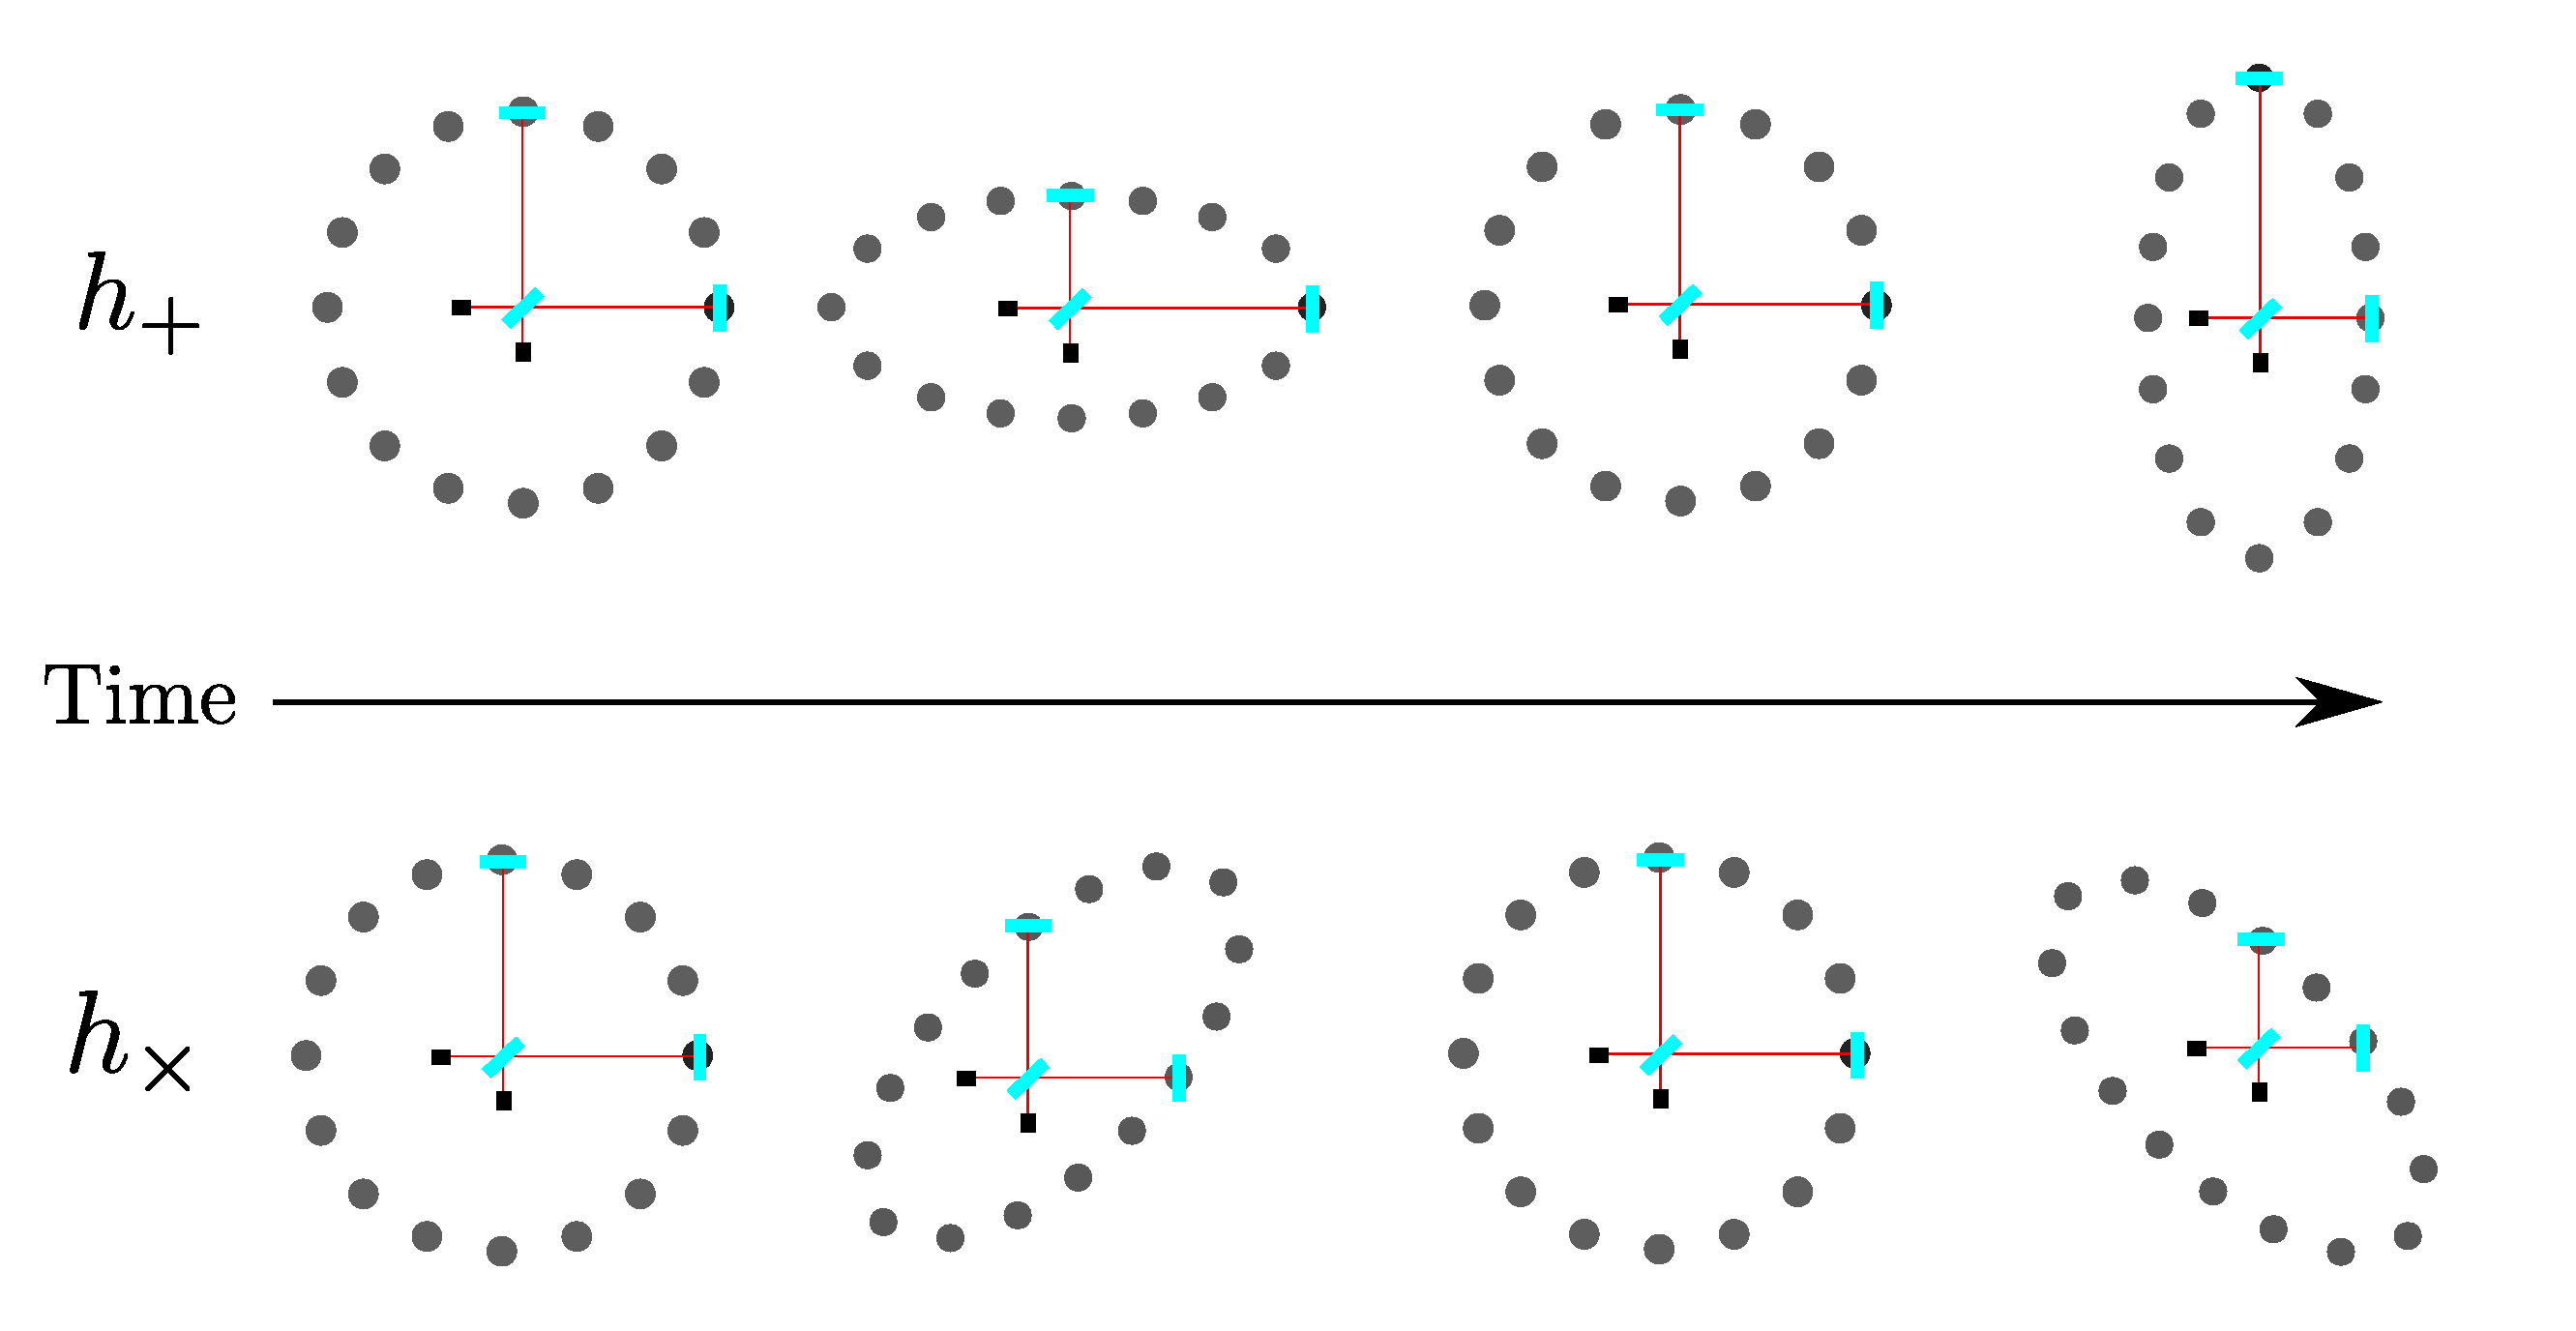
\includegraphics[width=\textwidth]{C1_intro/polarisation_ring.pdf}
    \caption[Plus and Cross polarisations]{Shows how the plus and cross polarisations affect a ring of test particles. This assumes the wave is travelling out of the page and the effects have been greatly exaggerated. This also shows an example of how this effects the test masses of an interferometer. This will be described in more detail in Sec.~\ref{intro:detector}.}
    \label{gw:polarisations}
\end{figure}



\subsubsection{Generating gravitational waves}

To generate gravitational waves we go back to Eq.~\ref{intro:lineinstein} where we include the stress-energy term on the right hand side.
Following the derivation in \citep{flanagan2005BasicsGravitational}, one can find that the gravitational wave amplitude is related to the second moment of the mass distribution.
The second moment of the mass distribution $I_{\mu\nu}$is defined as
\begin{equation}
    I_{\mu \nu}(t) = \int \rho(t,{\bf x}) x^\mu x^\nu d^3x,
\end{equation}
where $\rho$ is the mass density, and $x_i$ and $x_j$ are the coordinates \citep{flanagan2005BasicsGravitational}. 
This is the quadrupole moment tensor without the trace subtracted.
The gravitational wave amplitude is then
\begin{equation}
\label{intro:gravwave:amp}
    h_{\mu \nu} = \frac{2}{r}  \frac{d^2 I_{\mu \nu}(t-r)}{dt^2},
\end{equation}
where $r$ is the distance from the source \citep{letiec2016TheoryGravitational}.
This has a slight modification in the TT gauge, see \citep{flanagan2005BasicsGravitational}, however, has the same relationship between the mass quadrupole and the \gls{GW} amplitude.
This shows that for a \gls{GW} to be generated, the second derivative of the mass quadrupole moment is needed.
A mass quadrupole moment only exists when the mass distribution is not spherically symmetric.
Therefore, a mass which is asymmetric and accelerating will produce a \gls{GW}.

Systems which will produce detectable \glspl{GW} are generally rapidly rotating high mass systems which have some asymmetry around their rotation axis.
The sources of these \gls{GW} will be described in the following section.



%%%%%%%%%%%%%%
%%%%%%%%%%%%%
\section{\label{intro:sources}Sources and signals}
%%%%%%%%%%%%%%%
%%%%%%%%%%%%%%%

There are many potential sources for \gls{GW}. The expected sources can be split into 3 general categories based on their signal type: Transient, Stochastic and \glspl{CW}.
These categories are chosen based on the length of the signal and how well modelled the signal is.
Fig.~\ref{intro:sources:signaltypes} shows an example of each of the signals and their category.
%
\begin{figure}[h]
    \centering
    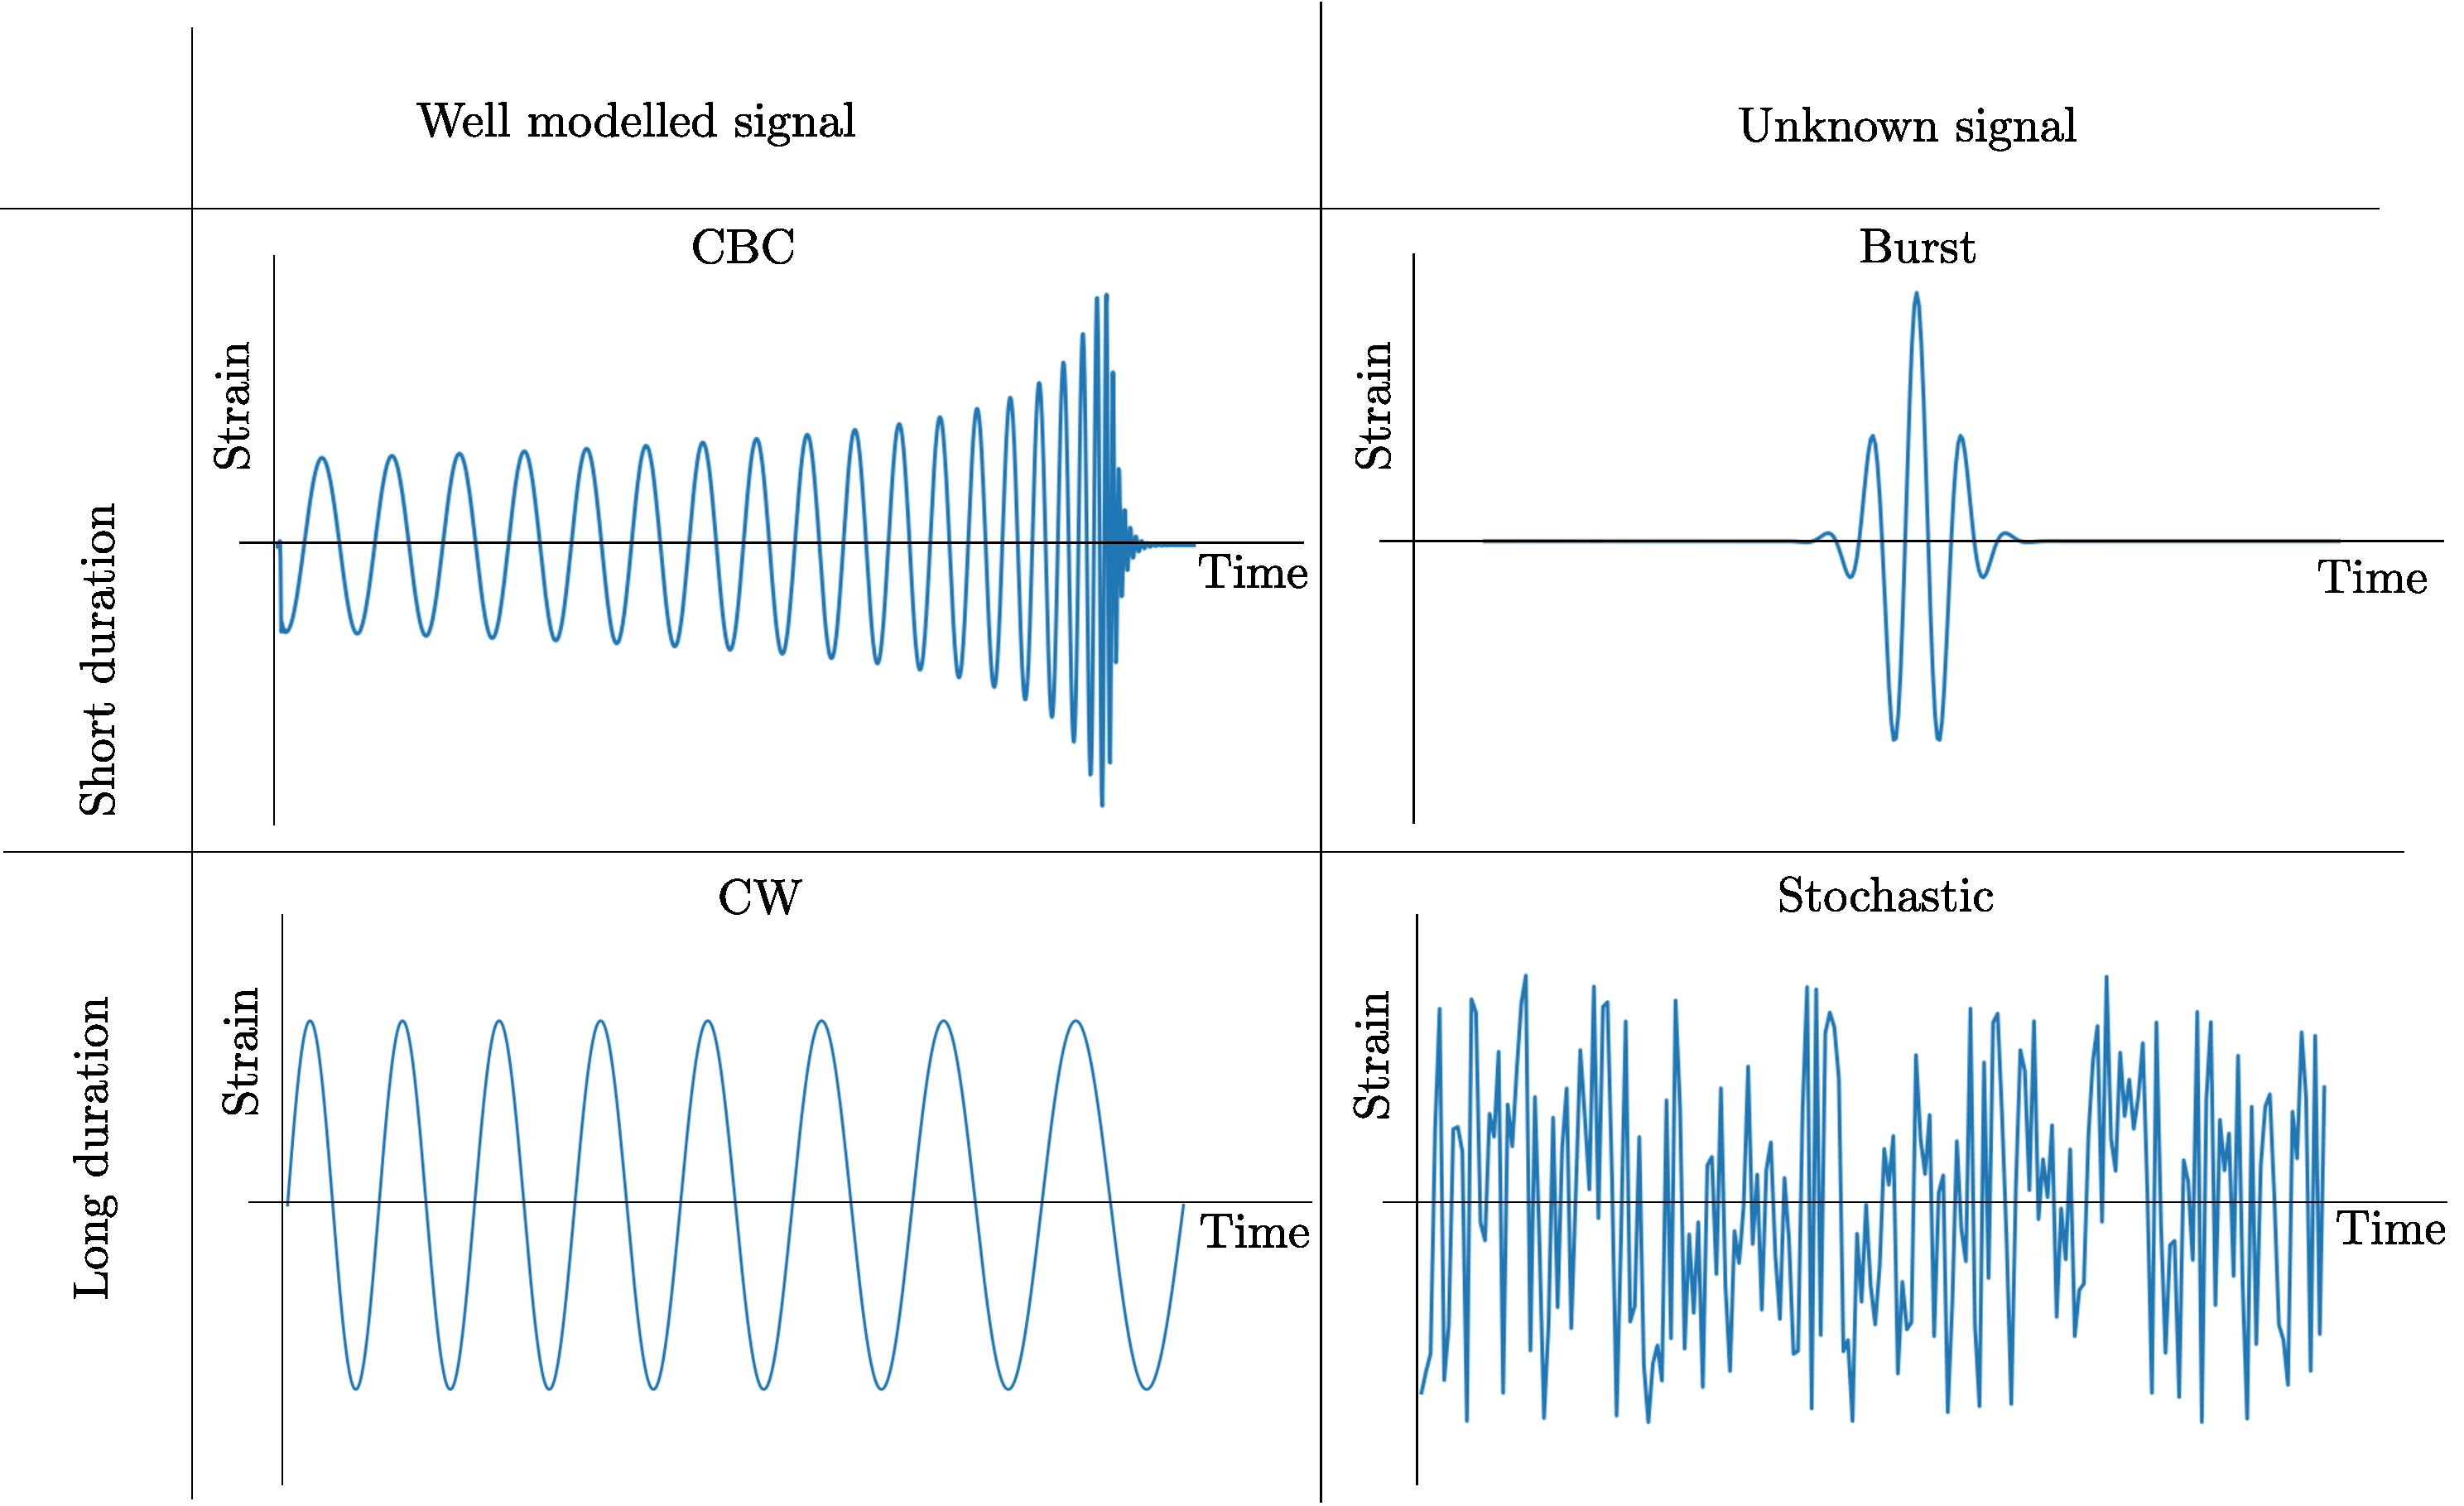
\includegraphics[width=\textwidth]{C1_intro/sources_types.pdf}
    \caption[GW signal types]{Each \gls{GW} signal type can be categorised based on its signal length and how well the signal is modelled. Transient signals which are short duration in the ground based detectors band, include both well modelled \gls{CBC} signals and unknown Burst signals. Long duration signals include well modelled \gls{CW} signals and unknown Stochastic signals.}
    \label{intro:sources:signaltypes}
\end{figure}
In the sections that follow, I will give an overview of the potential sources of each of these signal categories and their wave-forms.


%%%%%%%%%%%%%%%
\subsection{\label{sources:transient} Transient}
%%%%%%%%%%%%%%%

Transient sources of \glspl{GW} are short duration signals which are, depending on the source, observable from milliseconds to tens of seconds in current ground based detectors frequency band. 
Some of these sources, particularly \gls{CBC} sources, will emit signals for a much longer time, however these are at a lower frequency and not observable by current ground based detectors detectors.
Transient signals can be further split into two categories based on how well they are modelled. 
\glspl{CBC} have well modelled wave-forms and bursts are generally from un-modelled or unknown sources.

\subsubsection{\label{sources:transient:cbc} Compact Binary Coalescence}

\glspl{CBC} originate from the in-spiral and merge of two compact objects which are gravitationally bound.
The objects inspiral as they lost energy to the radiation of gravitational waves.
Dependent on the masses and distances of the two objects, the gravitational waves generated by the system can be detected by ground based detector such as LIGO \citep{aasi2015AdvancedLIGO} and Virgo \citep{acernese2015AdvancedVirgo}. 
In fact, the only detections to date have been of this type; these are summarised in \citep{ligoscientificcollaborationandvirgocollaboration2019GWTC1GravitationalWave}.

\joe{More qualatative, See Grahams comment}
The compact objects referred to here are either either black holes or neutron stars.
There are generally three types of \gls{CBC} source: \gls{BBH}, \gls{BNS} and \gls{NSBH}.
The general structure of the waveform is the same for each of these and follows a `chirp' where the \gls{GW} frequency increases with time until merger. An example of this is shown in Fig.~\ref{intro:sources:signaltypes}.
For higher mass systems such as \gls{BBH} these signals are detectable by ground based detectors for $< 1\,s$. 
For lower mass systems such as \gls{BNS} they can be detected for longer periods $\mathcal{O}(10)$s. 
The lower frequency parts of the signal (i.e. earlier times) aim to be detected by future space based detectors such as \gls{LISA} \citep{danzmann1996LISALaser}.

In systems which have a neutron star, during the in-spiral when the objects are \joe{find better word, close compared to what}close, the neutron star can deform due tidal interactions between the objects \citep{hernandezvivanco2019MeasuringNeutron,harry2018ObservingMeasuring}. 
This becomes useful as it will affect the generated waveform and can help place limits on and determine the \gls{EOS} for the dense matter in a neutron star \citep{hernandezvivanco2019MeasuringNeutron,harry2018ObservingMeasuring}.
\gls{BNS} systems also offer a way do observe objects in multiple different channels, or what is known as multi-messenger astronomy. 
This is where the object can be viewed in the \gls{EM} spectrum as well as in gravitational waves.
This offers much in the field of astronomy as it can aid in the measurement of the Hubble constant \citep{theligoscientificcollaborationandthevirgocollaboration2017GravitationalwaveStandard}. 
Observations of \gls{BBH} systems can also give information on how black holes and \glspl{BBH} form, more details on this can be found in \citep{zevin2017ConstrainingFormation,mandel2018MergingStellarmass}.


%%%%%%%%%%%%%%
\subsubsection{\label{sources:transient:burst}Burst}
%%%%%%%%%%%%%%%%%

Burst sources are also short duration however, are un-modelled or difficult to model, in the sense that the exact waveform of the signal is unknown.
There are two possible reasons for the lack in knowledge of the waveform: the physics of the system is too complicated to model in a reasonable amount of time or there is no model of the source.
As there is no model to generate waveforms, burst searches cannot use matched filtering as in \gls{CBC} searches.
Rather burst searches look for short bursts in power which is coherent between multiple detectors \citep{cornish2015BayeswaveBayesian, klimenko2008CoherentMethod} \joe{Check that search is actually coherent}.
There are a number of systems which could potentially emit a short duration burst signals.
These include core collapse supernovae \citep{ott2008GravitationalWave}, \glspl{GRB} \citep{aasi2014SearchGravitational}, cosmic strings \citep{damour2005GravitationalRadiation} and other unknown sources.
Detecting \gls{GW} from one of these sources could offer more insight into the processes which cause core collapse supernovae. 

As burst searches are un-modelled, they are sensitive to almost any signal which is coherent between detectors. 
This allows them to also search for signals from \gls{CBC} as well as any \gls{GW} signal from an unknown source.



%%%%%%%%%%%%%%%
\subsection{Stochastic}
%%%%%%%%%%%%%%%

The stochastic background has no signal model, however, is expected to be a persistent source of \gls{GW} in the background of the detector. 
The stochastic background is the incoherent sum of many unresolved \gls{GW} signals.
The source of these signals can be anything from cosmological sources such as cosmic strings to \gls{CBC} signals.
These signals can be thought of as the \gls{GW} analogue of the \gls{CMB}.
The signal is assumed to be isotropic such that it can be observed at any point on the sky \citep{christensen2018StochasticGravitational}. 
As the stochastic background is noise-like it is very difficult to distinguish from noise within a single detector \citep{christensen2018StochasticGravitational}.
Therefore, searches for the stochastic background correlate signals between multiple detectors \citep{romano2019SearchesStochastic,christensen2018StochasticGravitational}. 
When detected, these signals may be able to offer insights into the early universe and its formation.



%%%%%%%%%%%%%%%%%%
\subsection{\label{intro:sources:cw}Continuous waves}
%%%%%%%%%%%%%%%%%%%%

\glspl{CW} are long duration signals which can be well modelled.
The signals last for times greater than the observation runs of ground based detectors and in general have a fixed or slowly varying frequency.
There are a number or potential sources of \glspl{CW} including \glspl{CBC} long before their merger.
\joe{how long before, and rewite this sentance}Long before a \gls{CBC} merger, the two compact objects are orbiting each other whilst slowly inspiralling.
This will emit a long duration, almost fixed frequency sinusoid as its signal.
This signal however, is at lower frequency than ground based detectors can detect, therefore space based detectors such as \gls{LISA} \citep{danzmann1996LISALaser} are expected to observe this type of \gls{CW}.

The primary source for many \glspl{CW} searches is rapidly rotating neutron stars with spin periods ranging from $\sim 10^{-3} - 10$ s \citep{manchester2005AustraliaTelescope}.
Neutron stars originate when a massive \joe{how massive} star collapses and are the remnant of this collapse, they are objects with incredibly high density and are highly magnetised with field strengths of $10^8 - 10^{15}$ G \citep{konar2017MagneticFields}.
They have masses around $1.4-2 \; M_{\odot}$ contained in a star with radius of $\sim 10$ km.
Despite many observations in the electromagnetic spectrum and a large amount of research, these objects are not well understood.
A key part or neutron stars which is not understood is the \gls{EOS}. A review of the current understanding can be found in \cite{lattimer2016EquationState}.
The \gls{EOS} relates quantities such as the pressure and density of a neutron star and dictates how the neutron star matter behaves.
Observations of \glspl{GW} from neutron stars can place limits on the \gls{EOS} of this type of matter. 
These observations have already been made in the form of \gls{BNS} mergers \citep{abbott2017GW170817Observation}.
However, independent observations of rapidly rotating neutron stars can add to this understanding by placing limits on the deformability of the star and therefore the \gls{EOS}.

For a neutron star to emit a gravitational wave it needs to have some asymmetry in its mass distribution around its rotation axis, this follows from Eq.~\ref{intro:gravwave:amp}. 
There are a number of different mechanisms which could cause this and emit \glspl{GW}, some of these are reviewed in \citep{glampedakis2017GravitationalWaves,riles2017RecentSearches,haskell2015DetectingGravitational,lasky2015GravitationalWaves}.
Here I will summarise two main theories: Neutron star mountains and neutron star oscillations.


%%%%%%
\subsubsection{Mountains}
%%%%%%%%%

One of more likely mechanisms for detectable \gls{GW} emission from neutron stars is from `mountains' on the surface of the star.
These are permanent deformations of the crust which are non axisymmetric, i.e. the deformation is not symmetric around the rotation axis.

This deformation or asymmetry can be quantified by the ellipticity $\epsilon$ of the neutron star.
This is defined using the principal moments of inertial
\begin{equation}
\label{ellipticity}
\epsilon = \frac{I_{xx}-I_{yy}}{I_{zz}},
\end{equation}
where $I_{zz},I_{xx},I_{yy}$ are the principal moment of inertia.
This is when the star is rotating around the $z$ axis so $I_{zz}$ is along the rotation axis. 

There are a number of theories which describe the origin of this axisymmetry.
If the pulsar is in a binary system and accreting material from its companion star, the material can be funnelled towards the magnetic poles by the magnetic field, thereby causing a hot spot \citep{haskell2015DetectingGravitational}.
This `hot spot' could cause a deformation on the surface of the star which is not axi-symmetric. 
The magnetic stresses from strong magnetic fields within the star, could potentially also cause non axi-symmetric deformations to the star \citep{}.
Finally the spin down of the pulsar itself could cause stresses in the crust of the star until the point of breaking, its then after this break which could leave a distortion in the crust \citep{becker2009NeutronStars}.
More details on the signal waveform of this type of \gls{GW} and methods to search for it will be explained in Sec.~\ref{searchcw}.
 
 %%%%%%%%%%%%%%
 \subsubsection{Neutron star oscillations}
 %%%%%%%%%%%%%%%
 \joe{Probably shorten this section, as may not know enough to answer questions on}
There are a number of oscillation modes within a star such as f-modes, p-modes and r-modes \citep{becker2009NeutronStars}. 
Each of these waves are oscillations in the star similar to oscillations in the earth which measured in terrestrial seismology.
The difference between these modes is the restoring force bringing the perturbed state back to equilibrium.
For example, gravity is the restoring force for f-modes where the oscillations happen in the crust of the star.
The more promising of these for gravitational wave emission and detection is the r-mode \citep{lasky2015GravitationalWaves}. 
These are oscillations in the neutron superfluid part of the star, where the restoring force is the Coriolis effect from the rotation of the star.
Fig.~\ref{intro:source:cw:rmode} shows an highly exaggerated view of a neutron star with an oscillation mode travelling in each direction.
\begin{figure}[h]
	\centering
	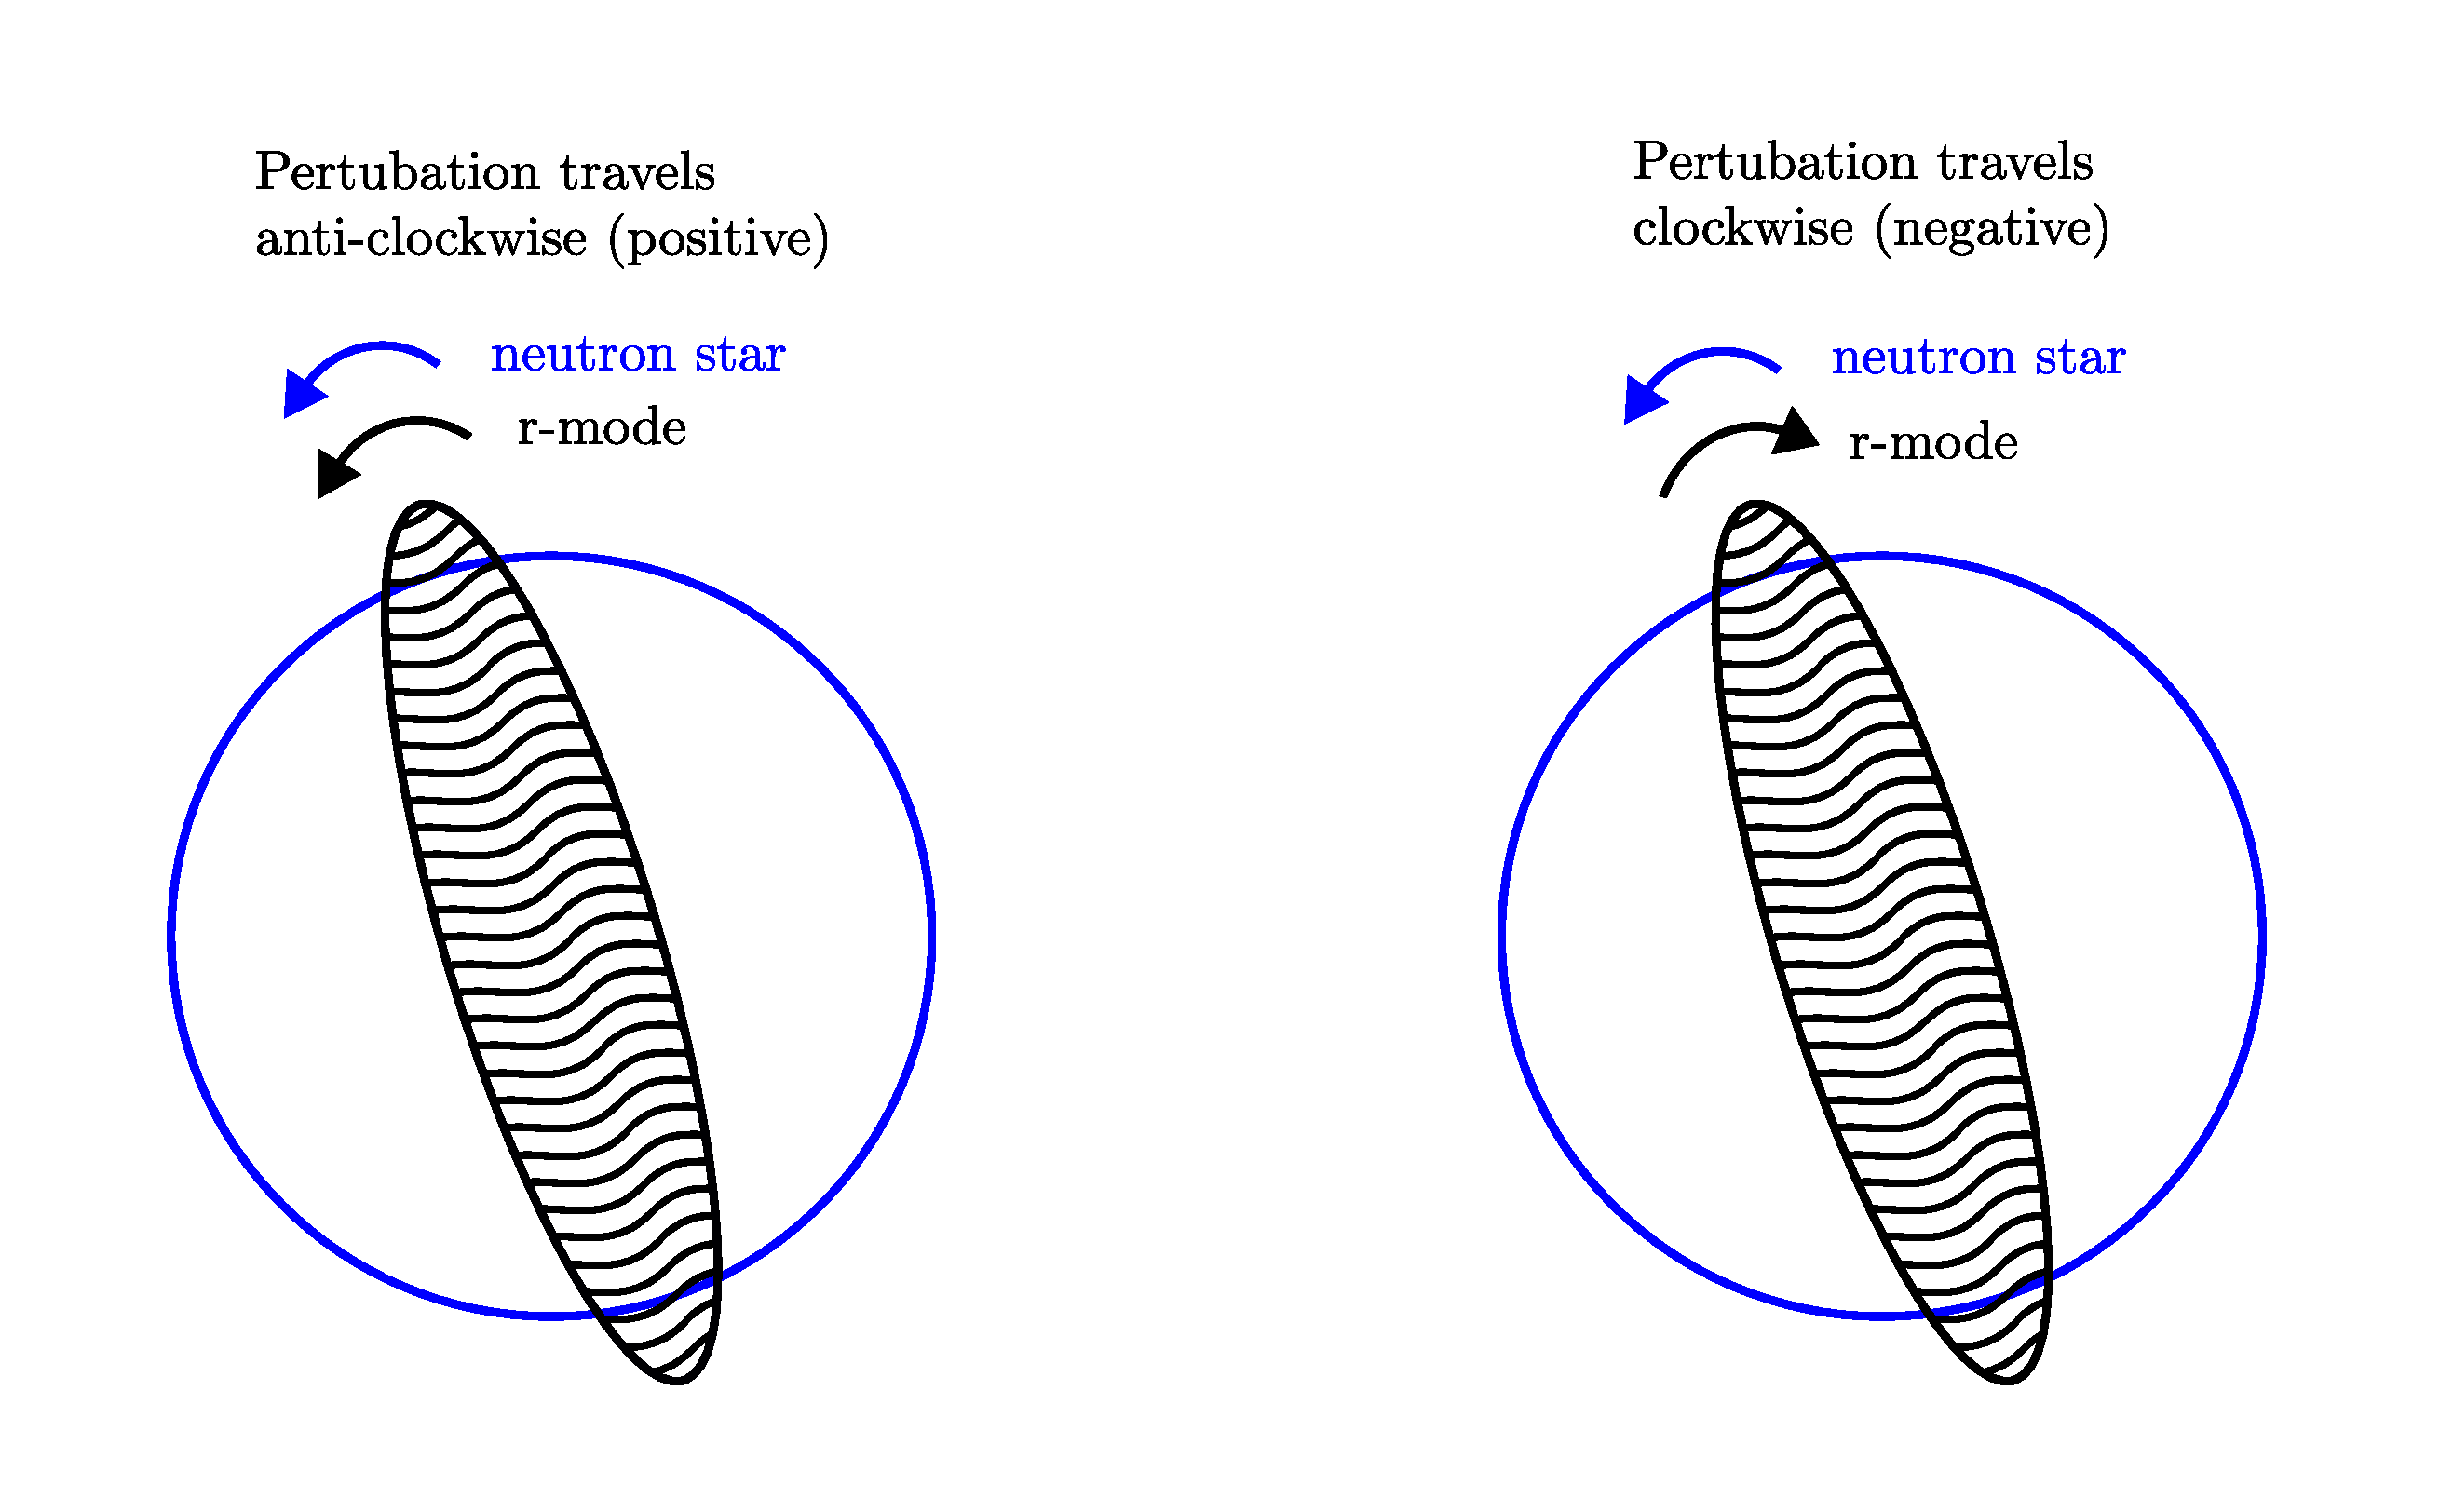
\includegraphics[width=\textwidth]{C1_intro/rmode.pdf}
	\caption[Generating \glspl{GW} from r-modes in neutron stars.]{The r-modes can travel in either direction in the star. in the case when the r-mode is moving clockwise and the neutron star is moving anticlockwise, if the neutron star is rotating fast enough it can cause unstable emission of \gls{GW}. This image was reconstructed from \citep{jonesCFSInstability}.}
	\label{intro:source:cw:rmode}
\end{figure}
If these modes are excited in a non-rotating star, then they will emit \gls{GW} where the \gls{GW}  carries away angular momentum \citep{jonesCFSInstability}. 
For the mode travelling in a clockwise direction, this angular momentum is positive and the mode travelling anti-clockwise the angular momentum is negative. 
Therefore, the \gls{GW} is taking away either positive or negative angular momentum (adding angular momentum) depending on the direction of rotation.
The emission of \gls{GW} damps the modes and the magnitude of the perturbation decreases making them extremely difficult to detect.
Now if the neutron star is rotating, this can lead to an effect called the \gls{CFS} instability  \citep{chandrasekhar1970SolutionsTwo,friedman1978SecularInstability}. 
As the rotation speed of the neutron star increases, there are two different effects on the modes travelling in opposite directions. 
For the mode travelling anti-clockwise with the stars rotation, the mode will appear to be travelling faster, therefore, will emit more \gls{GW} taking away more angular momentum. This means that this mode will be damped more rapidly.
The interesting affect is for the mode travelling clockwise, opposite to the neutron stars rotation. 
At a certain rotation rate, the mode will be `frozen' from the observers perspective and no \gls{GW} will be emitted.
As the rotation rate increases further, the mode will appear to travel anti-clockwise to an observer, i.e. the mode is dragged in the opposite direction by the stars rotation. 
Here it is key to remember that this mode had negative angular momentum as in the neutron stars frame it is still travelling clockwise.
As the mode rotates its emits positive angular momentum, which is then subtracted from the modes negative angular momentum.
The magnitude of the angular momentum then increases such that more \glspl{GW} are released.
This effect causes the amplitude of the oscillation to grow and therefore become unstable.
Therefore, a neutron star is unstable to \gls{GW} emission if it is rotating sufficiently fast \citep{lasky2015GravitationalWaves}.
For a more detailed view on how r-modes generate \gls{GW} see \citep{owen1998GravitationalWaves,jonesCFSInstability}


%%%%%%%%%%%%%%%
%%%%%%%%%%%%%%
%%%%%%%%%%%%%%%
\section{\label{intro:detector}Detectors}
%%%%%%%%%%%%%%%%
%%%%%%%%%%%%%%
%%%%%%%%%%%%%%

The indirect detection of gravitational waves from the Hulse-Taylor binary pulsar system left little doubt that \gls{GW} existed. 
The real challenge was to design an instrument which could directly detect gravitational waves.
There were a number of different proposed methods for the design of the instrument, notably: resonant bar detectors, both ground based and space based interferometers, pulsar timing arrays and cosmic microwave background (CMB) detectors. 
The first resonant bar detector was designed and built by Joseph Weber \citep{weber1966ObservationThermal}. 
These are large cylinders of metal which should resonate as a gravitational wave passes by. 
There are a few different designs of this type of detector, including an omni-directional design \citep{dewaard2003MiniGRAILFirst}. 
The majority of these detectors are no longer operational \joe{why}.
Pulsar timing arrays aim to use the accurate arrival time of pulses from millisecond pulsars to measure \gls{GW} \citep{hobbs2017GravitationalWave}. As a \gls{GW} passes between the pulsar and the observer, the arrival time of the pulses should change \joe{by how much}. 
Whilst a detection has not been made using pulsar timing arrays, these methods are still in use.
Cosmic microwave background detectors aimed to look for evidence of gravitational waves in the polarisation's of the CMB \citep{ade2018ConstraintsPrimordial}.  
These use the a range of detectors to look at the CMB however, are yet to confirm a detection of a \gls{GW} signal.
The most commonly known design of a \gls{GW} detector is the ground based interferometer, these made the first detection of \gls{GW} in 2015 \citep{abbott2016ObservationGravitational}. 
These are the focus of this section as the analysis that will follow uses data from the \gls{LIGO} detectors in the USA \citep{abbott2009LIGOLaser,aasi2015AdvancedLIGO} and Virgo detector in Italy \citep{acernese2015AdvancedVirgo,acernese2008StatusVirgo}. 

%%%%%%%%
%%%%%%%%%
\subsection{Laser Interferometers}
%%%%%%%%%%
%%%%%%%%%

Laser interferometers use the interference of light to measure a length with high precision.
The majority of this section will focus on ground based interferometers such as \gls{LIGO} and Virgo \citep{aasi2015AdvancedLIGO,acernese2015AdvancedVirgo}.
A simple design of an interferometer is shown in Fig.~\ref{detectors:interferometer:simple}. 
A laser beam is fired at a beam splitter which splits the light equally down two perpendicular arms. 
Each of these beams is reflected from a mirror at the end of either arm.
The light then returns to the beam splitter where the two beams are combined and sent to a photo-detector.
At the output, there is an interference pattern between the two beams.
If the length of one of the arms is changed then the interference pattern will change as the phase of one beam changes with respect to the other.
The phase difference of the light can be related to the wavelength of the light, $\lambda_l$ and the length of the detectors arms $L$ by
\begin{equation}
\label{intro:detectors:phasechange}
\Delta \phi \sim \frac{\Delta L}{\lambda_l},
\end{equation}
where $\Delta  \phi$ is the phase change and $\Delta L$ is the difference in the arm lengths \citep{}.
An interferometer can then measure small changes in the mirrors position.
\begin{figure}[hp]
    \centering
    \begin{subfigure}[h]{0.6\linewidth}
    	 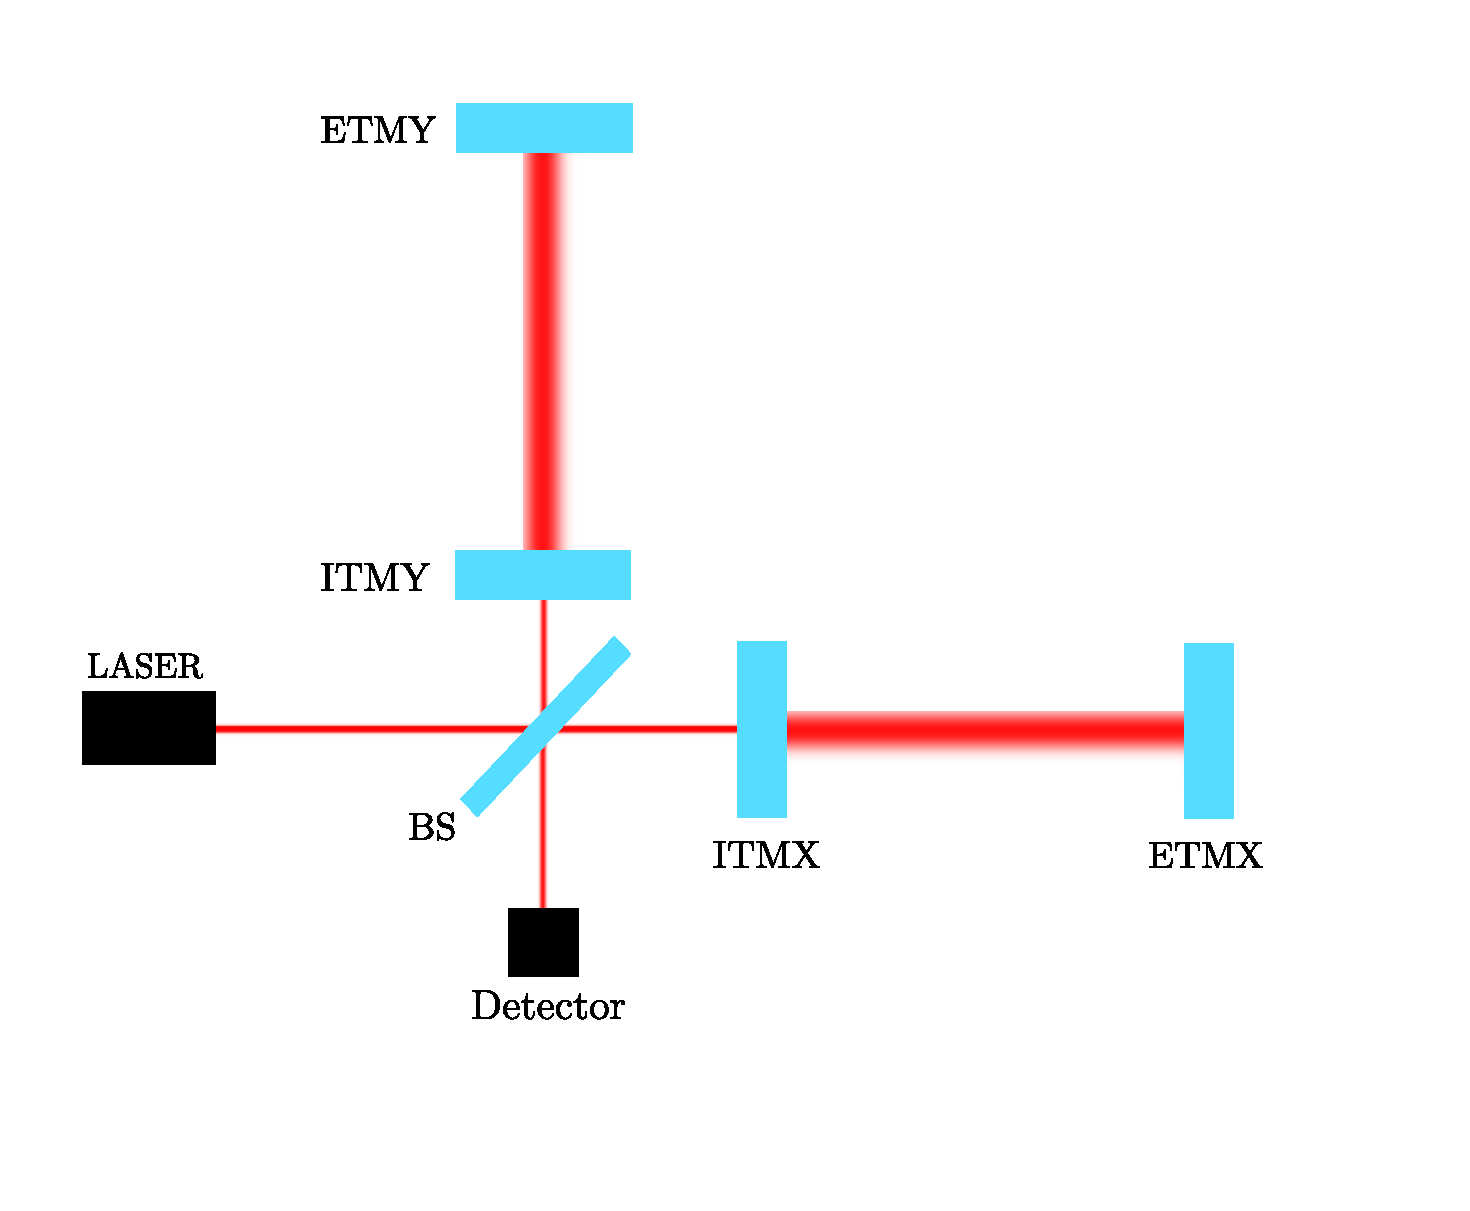
\includegraphics[width=\textwidth]{C1_intro/interferometer.pdf}
    	 \caption{Simple interferometer.}
    	 \label{detectors:interferometer:simple}
    \end{subfigure}
	\begin{subfigure}[h]{0.6\linewidth}
		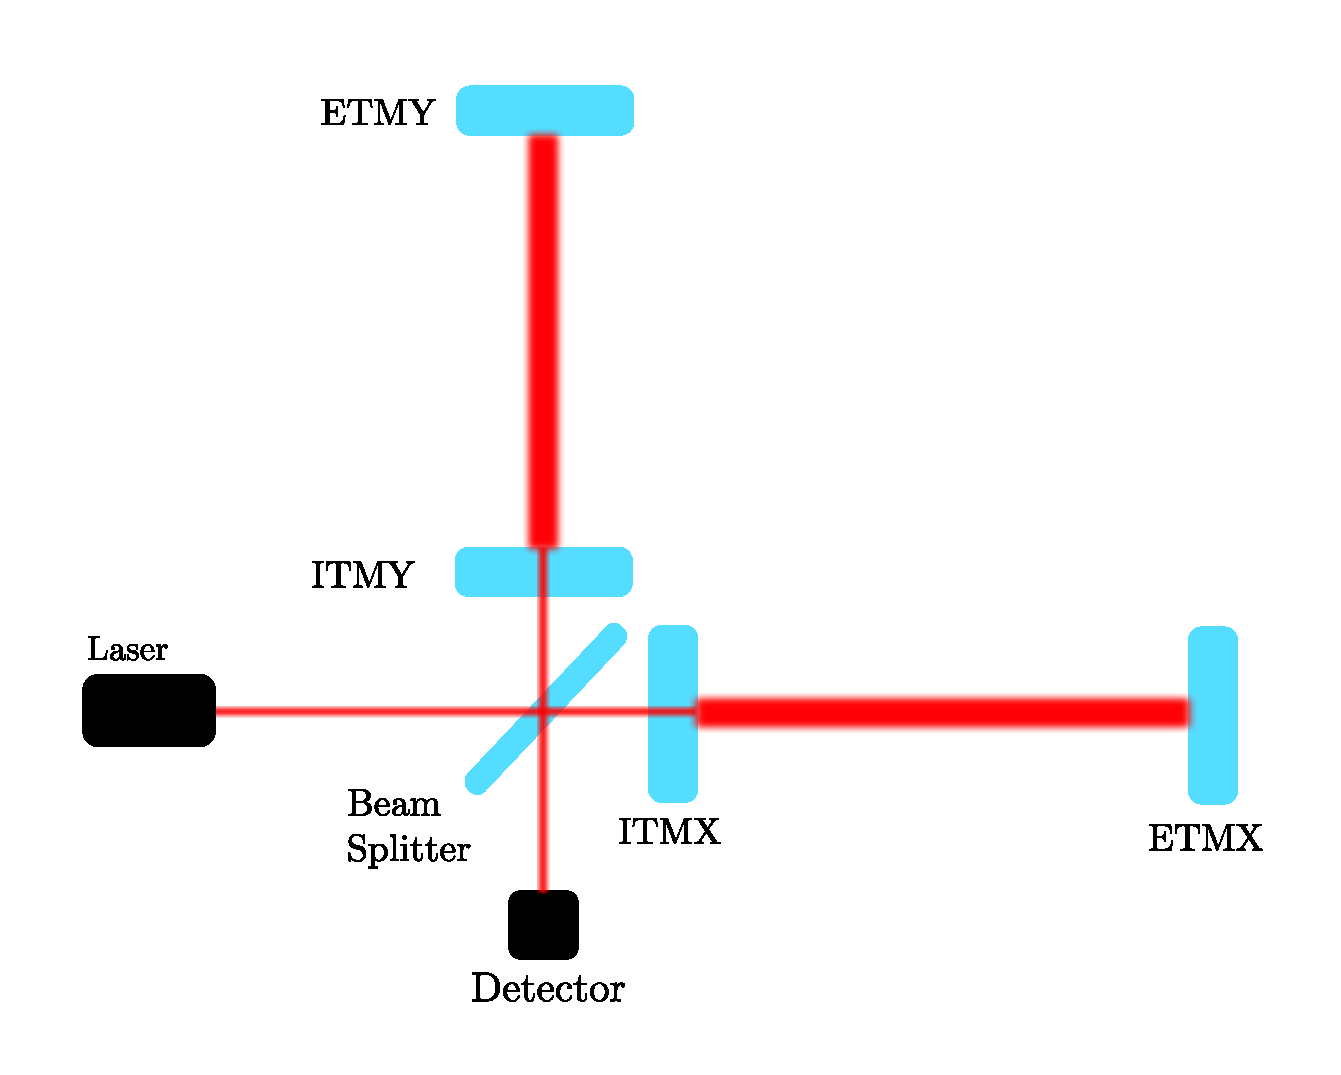
\includegraphics[width=\textwidth]{C1_intro/interferometer_fabry.pdf}
		\caption{Fabry-Perot interferometer.}
		\label{detectors:interferometer:fabry}
	\end{subfigure}
    \caption[Basic layout of the \gls{LIGO} detectors.]{\gls{LIGO} uses interferometry to make a detection. This has many additional features, one of which is shown above. ETMY and ETMX refer to the end test masses, which are just mirrors at the end of the interferometer arms. The beam splitter splits the Laser beam equally to each arm, this them recombines the beams back to the detector.
    ITMY and ITMX refer to the internal test masses, these create a Fabry-Perot cavity in the interferometers arms which can build up laser power. }
    \label{detectors:interferometer}
\end{figure}
%
This can be used in gravitational wave detection as the mirrors at the end of each arm of the interferometer can be treated as `free' test masses.
Fig.~\ref{gw:polarisations} shows the effect of a \gls{GW} in free test masses.
In the interferometer, this affect essentially changes the relative lengths of the two arms, i.e. $\Delta L$ in Eq.~\ref{intro:detectors:phasechange}.
The change of the interference pattern with time is then related to the \gls{GW}.
In practice the interference is held at a single point by adjusting the position of the two mirrors.
The \gls{GW} is then related to the readout of the mirrors control system.

If the mirrors at the end of the arms (ETMX and ETMY) are are placed further from the beam splitter, then the phase difference between the arms at the beam splitter for the same length change of one arm would be greater. 
This means that increasing the length of the detectors arms increases the sensitivity. 
A method to achieve a similar affect without physically increasing the arm length is to use a Fabry-Perot cavity \citep{aasi2015AdvancedLIGO}, this is shown in Fig.~\ref{detectors:interferometer:fabry}.
This is where a semi-transparent mirror is placed between the beam splitter and end mirror in each arm (ITMX and ITMY).
Light enters this cavity and reflects back and forth between the two mirrors (ITMX and ETMX) a number of times before returning to the beam splitter.
This increases the time the light spends in one arm and is equivalent to increasing the arm length.
Actual ground based \gls{GW} detectors such as \gls{LIGO} \citep{abbott2009LIGOLaser} and Virgo \citep{acernese2015AdvancedVirgo} are much more complicated than described above.
They use many techniques to increase the sensitivity some of which are outlined in \citep{aasi2015AdvancedLIGO,abbott2009LIGOLaser}.
Many of these techniques are designed to reduce non-astrophysical affects on the detector, some of these effects and solutions are listed in Sec.~\ref{intro:detector:noise}.



%%%%%%%%%%%
%%%%%%%%%%
\subsubsection{Detector response}
%%%%%%%%%%
%%%%%%%%%

An important factor to know when using detector data to search for astrophysical signals is the detectors response.
This measures how sensitive the detector is to different directions.
An example of the antenna response for \gls{LIGO} is in Fig.~\ref{intro:detectors:response} where the detectors arms lie on the x and y axis of the image.
This is clear when thinking about how a gravitational wave affects the test masses as in Fig.~\ref{gw:polarisations}. 
As the \gls{GW} is transverse to its propagation, when the detector is face on to the source, there will be a maximum change in the arm lengths and therefore a maximum sensitivity. 
In the same way the sensitivity will be at a minimum when edge to the source.

\begin{figure}
    \centering
    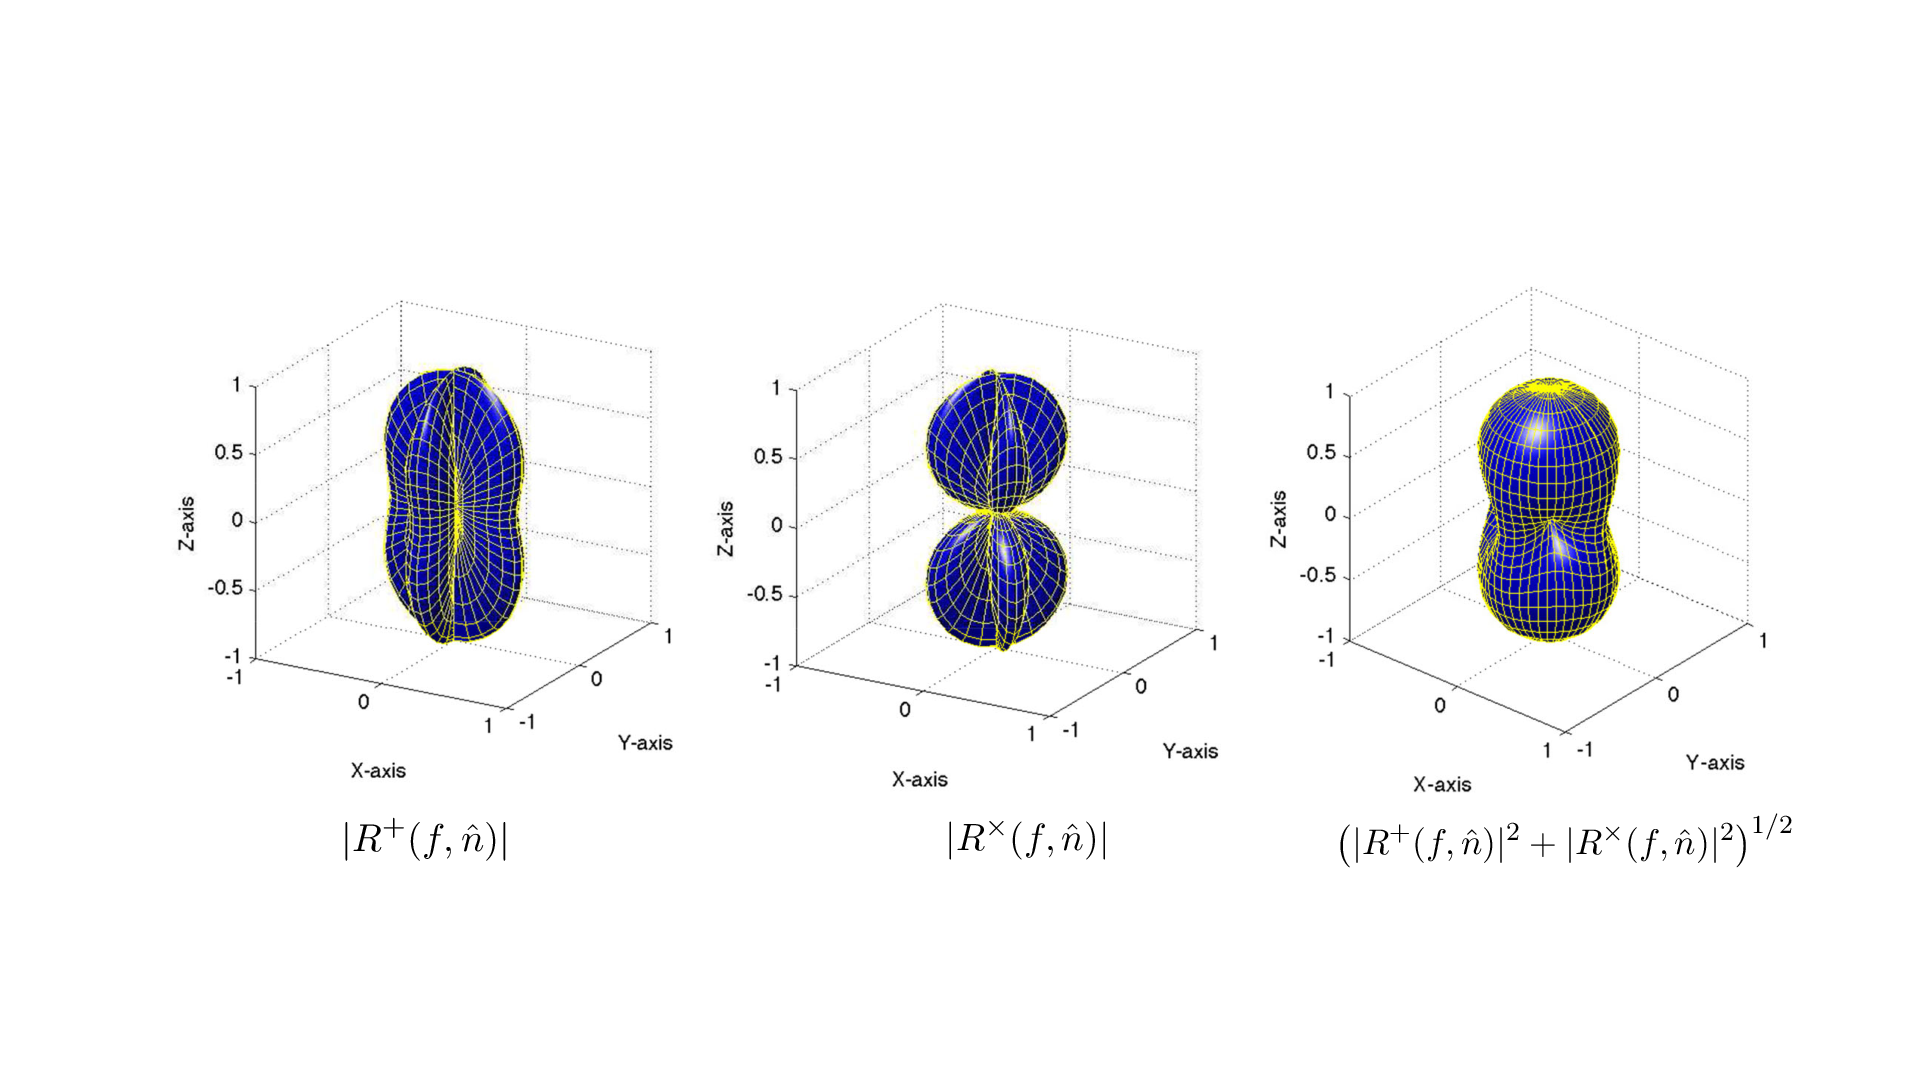
\includegraphics[width=\textwidth]{C1_intro/LIGO_beam_patterns.png}
    \caption[Antenna response of the \gls{LIGO} detectors.]{The antenna response is shown as in \citep{romano2019SearchesStochastic} for the plus, cross and average polarisation's. The detectors arms lie on the x and y axis in the above plots. }
    \label{intro:detectors:response}
\end{figure}

%%%%%%%%%%%
%%%%%%%%%%
\subsubsection{\label{intro:detector:noise}Noise sources}
%%%%%%%%%%
%%%%%%%%%%

To increase the sensitivity of the \gls{LIGO} detectors, any effect on the output of the interferometer which is not astrophysical ideally needs to be reduced.
This involves understanding what causes certain noise features in the detector, and how the affect of these can be limited. 
Within the detector, there are many sources of noise.
Some of these noise sources and how they limit the detectors strain sensitivity are all shown in Fig.~\ref{detectors:noisesensitivity} from \citep{aasi2015AdvancedLIGO}.
\begin{figure}[h]
    \centering
    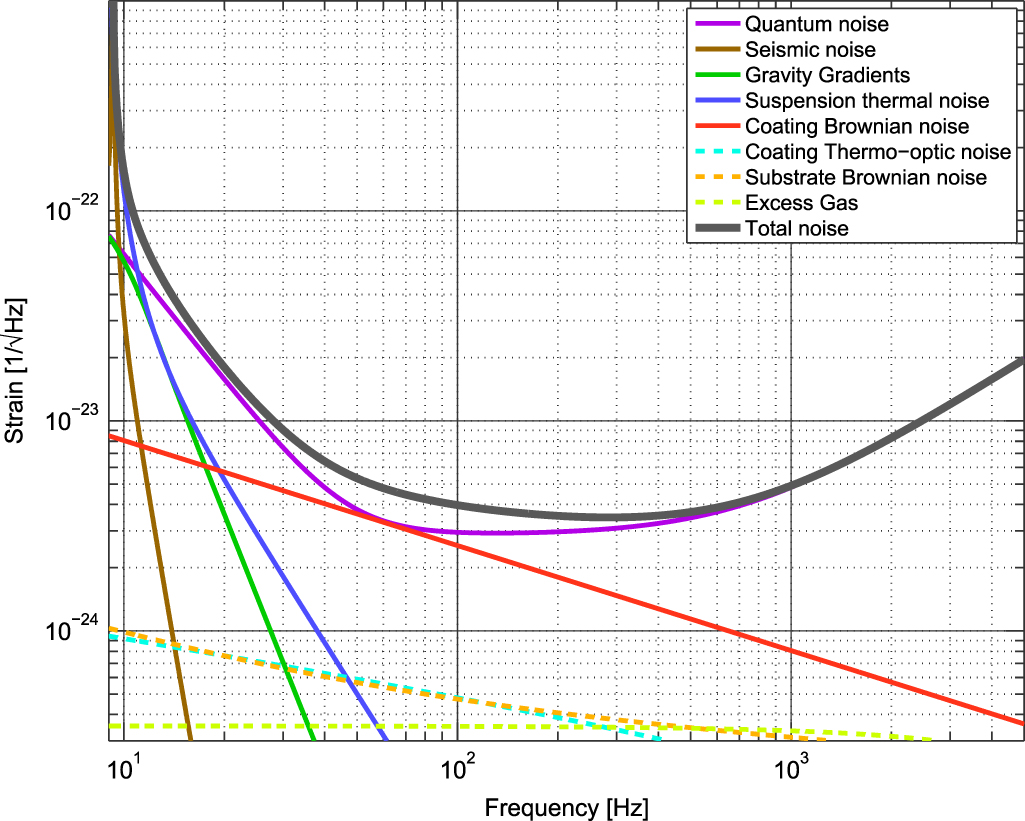
\includegraphics[width=0.9\textwidth]{C1_intro/noise_sensitivity.jpg}
    \caption[Example strain sensitivity curves for different noise sources in \gls{LIGO}.]{The different noise sources affect the sensitivity of the \gls{LIGO} detectors at different frequencies. This shows the various sources how the affect the noise curve \citep{aasi2015AdvancedLIGO}.}
    \label{detectors:noisesensitivity}
\end{figure}
Here I will summarise some of the limiting sources and also sources which become useful for understanding later sections.

\begin{description}
\item[Seismic noise] This originates from the seismic activity of the earth and effects lower frequencies. This can be oscillations such as earthquakes or ocean waves. Seismic waves cause the mirrors to oscillate and induce a change in the length of the arm. This is reduced by having multi stage suspensions in the detectors which essentially absorb the seismic oscillations \citep{matichard2015SeismicIsolation}.

\item[Coating noise] This is in general due to two main factors, the thermal noise of the coating and Brownian noise. The Brownian noise is from the mechanical dissipation in the coating and the thermal noise is due to thermal dissipation. The Brownian noise is the dominant factor as shown in Fig.~\ref{detectors:noisesensitivity}. These effects are limited by using different coatings on the mirrors \citep{abernathy0OverviewResearch}.

\item[Quantum noise] Quantum noise is a fundamental limit due to the statistical uncertainty of counting photons. This limits the sensitivity at many frequencies.There are methods to reduce this include squeezing of the light \citep{aasi2013EnhancedSensitivity}. 

\item[Electronics noise] Whilst this is not shown in Fig.~\ref{detectors:noisesensitivity}, this becomes important to searches described later. These have a different effect on the detector which is more narrowband frequency lines. This is generated by the digital and analogue electronics that are used to measure the signal. 
\end{description}

There are also many other sources of noise in the detector which I have not listed. However, these are often not the limiting cases of noise or are not relevant to this thesis.
In Sec.~\ref{detchar} I will go into more detail about specific noise sources in the detector known as instrumental lines and how they can be monitored and potentially removed. 












